\documentclass[10pt,letterpaper]{article}
\usepackage[margin=.85in]{geometry}
\usepackage[T1]{fontenc}\usepackage{lmodern,graphicx,booktabs,amsmath,xcolor,hyperref,xurl,caption,fancyhdr}
\hypersetup{colorlinks=true,urlcolor=teal,linkcolor=teal,pdftitle={Evaluate GDP forecasts with the data available then},pdfauthor={James Jean}}
\pagestyle{fancy}\fancyhf{}\fancyhead[L]{\small GDP vintage audit / Study 24}\fancyhead[R]{\small Independent retrospective study}\fancyfoot[C]{\thepage}
\setlength{\headheight}{14pt}\setlength{\parindent}{0pt}\setlength{\parskip}{6pt}\captionsetup{font=small,labelfont=bf,hypcap=false}
\begin{document}
{\small\color{teal} ECONOMIC FORECAST EVALUATION / INFORMATION AVAILABLE AT THE ORIGIN\par}
\vspace{7pt}{\LARGE\bfseries Evaluate GDP forecasts with the data available then\par}
\vspace{6pt}James Jean \hfill 30 October 2026
\section*{The decision}
A reviewer comparing economic forecasts needs two dates: when the model's input information was available and which GDP estimate is used to judge it. Substituting revised history can change the prediction; substituting a revised target can change its score. This study separates those effects using the Philadelphia Fed's real-time GDP archive.

\textbf{Finding.} The development-selected half-mean, half-latest-growth rule does not beat a plain twenty-quarter mean on the 42 eligible held quarters. With origin-vintage inputs and early targets, their MAEs are \textbf{3.629 and 2.987 annualized percentage points}. Keeping those predictions and using the 2026Q3 target changes MAEs to \textbf{3.641 and 3.012}. The mean remains ahead. All six rules, both input vintages and both target vintages remain visible below.

\textbf{Practical recommendation.} Require a vintage identifier for inputs and targets, retain the original forecast export, and review simple baselines before accepting an improved backtest. An error measured against a later GDP estimate is a different evaluation from an error against the early release. A revised-input backtest does not establish a forecast that could have been made at the time.

\begin{center}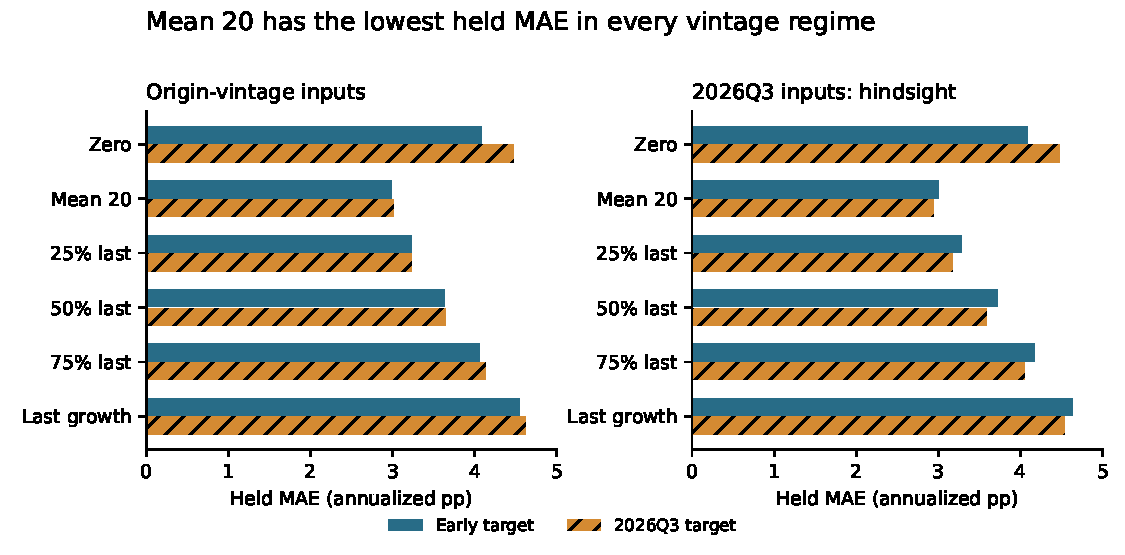
\includegraphics[width=\linewidth]{images/all_candidates.pdf}\end{center}
\captionof{figure}{Held MAE in annualized percentage points, 42 common eligible quarters. Every bar starts at zero. The revised-input panel deliberately uses hindsight. The twenty-quarter mean has the lowest MAE in all four regimes; no selected-model victory is claimed.}

\textbf{Important limits.} This is a corrected source-interpretation retrospective benchmark, not a prospective or untouched preregistered experiment. Exact-day historical access is unknown. The separate First series agrees at its observed stored precision, not beyond it. No investment return, deployment, significance result or operational benefit is established.
\newpage
\section*{1. Sources, timing and the precision correction}
Two official Philadelphia Fed files supply quarterly real-output levels by vintage and separate First/Second/Third growth releases [1--3]. The public subset contains 2,323 selected factual numeric cells and 102 vintages; original workbooks remain privately retained. Source coordinates, original-file hashes, exact capture requests and a minimal projection manifest preserve provenance. A separate OOXML reader reconciled every selected cell and independently scanned each selected vintage's last observation: 45,528 checks. Public reproduction verifies the captured projection's hashes and schema; it does not re-download or independently relicense the source.

Source documentation describes quarterly vintages in February, May, August and November. A target quarter's origin vintage must end at the previous quarter; the next quarter's vintage supplies the early target. This supports a mid-quarter snapshot experiment, not a trading-day simulation. Revised inputs and revised targets use the fixed 2026Q3 vintage, which was deliberately unavailable at historical origins. It is one later estimate, not final truth. Definition changes as well as additional measurement can contribute to revisions [2].

\begin{center}\begin{tabular}{lrr}\toprule
Role & Planned quarters & Eligible scored quarters\\\midrule
Development, 2000Q1--2011Q4 & 48 & 48\\
Separation, 2012Q1--2013Q4 & 8 & 0\\
Held, 2014Q1--2024Q4 & 44 & 42\\\bottomrule
\end{tabular}\end{center}
The separation block is deliberately unscored; documentation exposed 2012 examples before collection. Already-available separation-period observations may later enter lag histories. Two government-shutdown timing exceptions were excluded before collection: 2018Q4 as a target and 2019Q1 as an origin. All 100 planned origins remain in the ledger. No missing history was interpolated or converted to zero; all other planned origins met the source rules.

Within one vintage, annualized growth is
\[g_t=100\left[\left(\frac{GDP_t}{GDP_{t-1}}\right)^4-1\right].\]
Require 21 positive consecutive levels for 20 available lagged growth rates. Computing both levels within the same vintage avoids splicing differently rebased dollar series. Model growth is rounded half-even to twelve decimal places; predictions and losses then use exact rational arithmetic. Twelve computational places do not imply twelve-digit economic accuracy. RMSE uses a fifty-digit decimal square root before display.

\textbf{Recorded correction.} The original comparison of full-rational level growth against the separately supplied First series failed for all 98 non-exceptional targets. Inspection found that First cells store at most four decimal places, while Excel displays three. The documentation does not promise higher precision. Before any forecast score, the check was corrected to compare exact four-decimal half-even growth with the stored First value, retaining the original $10^{-8}$ residual threshold and all raw differences. All 98 then agreed. Original failed code, protocol and output were retained privately; the public protocol records the change. Higher-precision First agreement remains unverified. This changes source representation, not targets, candidates, temporal split or exclusions.
\newpage
\section*{2. Six fixed rules and development selection}
For each target, let $m$ be the mean of the twenty available lag growth rates and $\ell$ the latest available growth rate. Candidate zero predicts zero. The other five predict $(1-w)m+w\ell$ for fixed weights $w=0,1/4,1/2,3/4,1$. These are simple deterministic benchmarks, not fitted autoregressions, optimized hyperparameters or new estimators. The grid, history length and zero comparator were declared before source collection. There is no random seed, feature search or imputation.

Selection uses equal-quarter development MAE separately in each vintage regime. Exact MAE ties prefer the lower candidate index. The same fifty-percent blend wins in all four development comparisons. All candidates remain in the table; RMSE and squared losses remain in the machine-readable exports. MAE is in annualized percentage points, MSE in squared percentage points and RMSE in percentage points.

\begin{center}\small\begin{tabular}{lrrrr}\toprule
 & Origin/early & Origin/later & Revised/early & Revised/later\\\midrule
Zero & 2.769 & 2.773 & 2.769 & 2.773 \\
Mean 20 & 1.955 & 2.199 & 1.947 & 2.222 \\
25\% last & 1.702 & 2.006 & 1.661 & 2.032 \\
50\% last & 1.595 & 1.983 & 1.527 & 2.024 \\
75\% last & 1.627 & 2.043 & 1.593 & 2.276 \\
Last growth & 1.765 & 2.171 & 1.936 & 2.606 \\
\bottomrule\end{tabular}\end{center}
\textbf{Table 1.} Development MAE on the same 48 quarters in each column. ``Later'' means target vintage 2026Q3; ``revised'' means input vintage 2026Q3. Hindsight inputs are experimental controls.

\begin{center}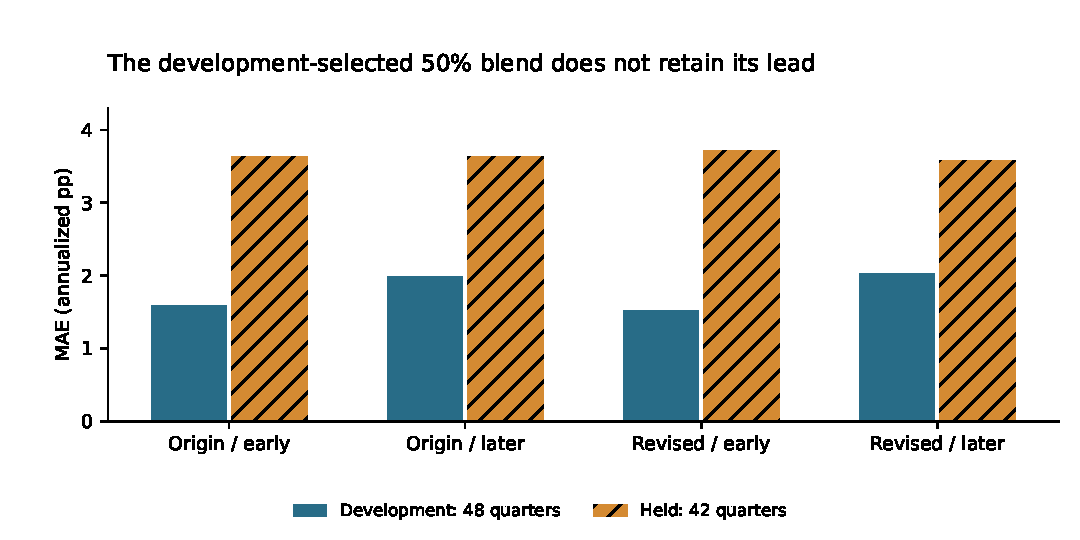
\includegraphics[width=.97\linewidth]{images/selected_transfer.pdf}\end{center}
\captionof{figure}{The selected blend's development and held MAEs. Different periods are not exchangeable samples: the held period includes pandemic shocks. This comparison describes transfer failure of the fixed development choice; it does not isolate a causal mechanism.}

After development verification, twenty-six dependency hashes were committed and pushed in freeze revision \texttt{5dbc870}. They bind the source projections, protocol including its precision correction, transformation and benchmark code, independent checker, synthetic fixtures, eligibility, development predictions and selection. The first held execution records this revision. Held outcomes do not change the candidate family, metric, eras or selected rule. Source values and historical economic events were not claimed to be blinded.

The four regimes hold origins, lag length, rules and cohort constant. A target-only contrast keeps predictions identical and changes only the evaluation target. An input-only contrast keeps its target fixed while recomputing predictions from revised histories. Combining these changes into one headline would hide what caused a score difference.
\newpage
\section*{3. Held results and what revisions actually change}
\begin{center}\small\begin{tabular}{lrrrr}\toprule
 & Origin/early & Origin/later & Revised/early & Revised/later\\\midrule
Zero & 4.090 & 4.475 & 4.090 & 4.475 \\
Mean 20 & 2.987 & 3.012 & 3.003 & 2.939 \\
25\% last & 3.234 & 3.226 & 3.284 & 3.167 \\
50\% last & 3.629 & 3.641 & 3.716 & 3.584 \\
75\% last & 4.058 & 4.131 & 4.174 & 4.046 \\
Last growth & 4.548 & 4.622 & 4.636 & 4.543 \\
\bottomrule\end{tabular}\end{center}
\textbf{Table 2.} Held MAE on 42 common eligible quarters, 2014--2024. The twenty-quarter mean wins each column after the development-selected blend is fixed. This is a descriptive held ranking, not a new held-based selection for deployment.

The selected blend's RMSE is 9.511, 9.384, 9.231 and 9.075 in the same column order. RMSE is much larger than MAE because a few large errors have greater weight under squared loss. Both losses remain visible; no extreme quarter is removed to make the model look better.

\textbf{Changing targets.} With origin-vintage inputs, the selected blend's MAE rises by about 0.012 percentage point when the target moves from the early estimate to 2026Q3. The mean's MAE rises by about 0.024. These are descriptive paired absolute-loss differences on the same quarters; the forecasts themselves do not change. Revisions can increase or decrease scores for other rules, as the full contrast export shows.

The full six-rule ordering has no strict pairwise reversal across target vintages with origin-vintage inputs. With revised inputs there is one reversal among fifteen pairs: zero versus the seventy-five-percent blend. Their MAEs change from 4.090 versus 4.174 against the early target to 4.475 versus 4.046 against the later target. The lowest-MAE rule stays the twenty-quarter mean. No target-induced tie transitions occur in these two input settings. The study therefore does not support a sweeping claim that vintage choice always changes the preferred model.

\textbf{Changing inputs.} Holding the early target fixed, the selected blend moves from MAE 3.629 with origin-vintage history to 3.716 with revised history. Holding the later target fixed, it moves from 3.641 to 3.584. Revised inputs are not uniformly favorable here. A researcher should report each controlled contrast rather than assume that hindsight always lowers an error.

Each candidate has complete prediction, exact absolute-loss and squared-loss exports. Annual summaries for every held year and the fixed eras on the next page retain the original denominator. All four development choices happen to agree; this agreement does not make revised inputs historically available or the development winner a held winner.

These findings concern one univariate rule family and one fixed later vintage. They do not compare full professional forecasting systems, survey expectations, nowcasting indicators or decision-specific loss functions. A broader vintage-sensitivity claim needs additional datasets and predeclared cohorts. No post-outcome parameter search or new experiment is represented as part of this release.
\newpage
\section*{4. Time variation and uncertainty}
The held set is small, temporally ordered and serially dependent. A pooled score can conceal very different periods. The fixed era summaries below use origin-vintage inputs and early targets; annual and all-regime summaries remain in the exports. Excluded quarters remain in the source ledger, not in a favorable replacement sample.

\begin{center}\small\begin{tabular}{lrrrrr}\toprule
 & $n$ & Mean MAE & Mean RMSE & Blend MAE & Blend RMSE\\\midrule
2014-2019 & 22 & 0.912 & 1.093 & 0.930 & 1.211 \\
2020-2021 & 8 & 11.338 & 17.363 & 14.259 & 21.537 \\
2022-2024 & 12 & 1.226 & 1.820 & 1.488 & 2.173 \\
\bottomrule\end{tabular}\end{center}
\textbf{Table 3.} Equal-quarter losses in annualized percentage points. ``Blend'' is the development-selected fifty-percent rule. Era boundaries were fixed before collection; the two timing exclusions reduce the first era to twenty-two quarters.

\begin{center}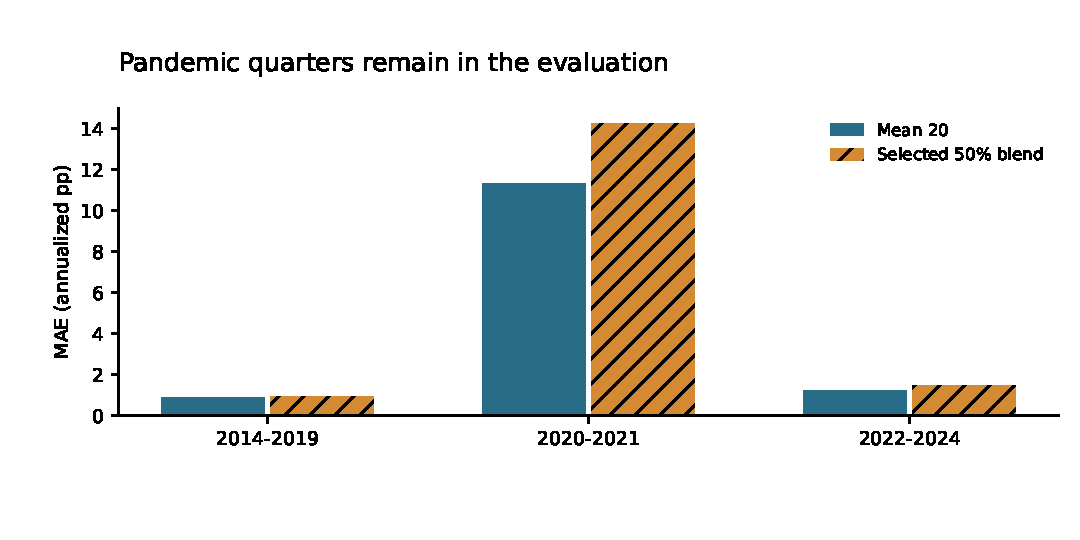
\includegraphics[width=.98\linewidth]{images/era_context.pdf}\end{center}
\captionof{figure}{Pandemic-period errors dominate the overall MAE. All eight 2020--2021 quarters are retained. The selected blend has higher MAE in all three fixed eras under this regime; the magnitude of that gap varies substantially.}

There is no independent sampling design, randomization or stable-error assumption that would justify a universal confidence interval. The paper reports exact descriptive paired differences for this finite cohort. It does not attach an invented significance level to the rankings, treat annual observations as independent replications, or infer causality from a change of data vintage.

Source rounding and changes in GDP measurement are additional limits. The four-decimal First comparison checks consistency with the stored source representation; the level-based model target uses the separately declared twelve-place computational representation. Neither is a physical ground truth. Quarterly vintage documentation supports snapshot information boundaries but not exact-day operational access or a live data delivery guarantee.

\textbf{Decision implication.} Keep the simple mean in a model review, preserve the historical input snapshot and state the target vintage explicitly. Before using a forecast for a real decision, define its timing, available predictors and actual loss. This study supplies audit evidence and a reproducible comparison; it measures no financial or policy benefit.
\newpage
\section*{5. Reproduction, prior work and next use}
Real-time data and revision-sensitive forecast evaluation are established subjects, including Croushore and Stark's RTDSM research [4,5]. This work offers a small transparent implementation and controlled comparisons, not a new forecasting estimator or a claim of scientific priority. No exhaustive novelty search or external peer review has been completed.

The separate source reader used workbook XML rather than the projection reader's openpyxl path. Independent result verification uses SQLite joins, 160-digit Decimal growth and exact rational losses without importing the analysis helpers. It checked 22,320 development and 22,565 held assertions, including all 100 origins, 4,000 growth inputs, 1,152 development predictions, 1,008 held predictions, all rankings, contrasts, pairwise orders and fixed subgroup metrics. These finite checks do not establish universal correctness.

Twenty-three synthetic fixtures cover date rollover, invalid dates, growth annualization, rebasing invariance, signed half-even rounding, short histories, positive-level requirements, zero losses, exact ties, future/stale information, target binding and source-precision failure. Fixtures are invented interface/arithmetic cases, excluded from research outcomes.

Offline reproduction uses a temporary local Git clone, rebuilds transformations and predictions, runs independent checks and the fixtures, and compares 63,116 CSV fields and five JSON documents exactly. Original exports remain unchanged; no new source request occurs. Figure verification checks 38 source values, 304 actual SVG rectangle coordinates and nine artifact hashes. Manuscript displays are independently rebuilt from prediction exports, followed by PDF structure and rendered-page checks. Later exact-candidate and main Linux successes, tested/merged-tree equality and a verified annotated remote tag are release requirements; local manuscript evidence alone does not assert those later gates passed.

\textbf{Run locally.} Use Python 3.12 and install \texttt{requirements.txt}. Run \texttt{python src/reproduce.py}, then the figure, paper and canonical-Git checks named in the workflow. Full original-source reconciliation additionally needs the retained private workbooks. The source supports informational, educational and research use subject to its terms and underlying rights [6]; the public repository contains attributed minimal factual projections, not the raw compilation, logos or source documents. No blanket CC0, endorsement or commercial-service rights are claimed.

\textbf{Next use.} Apply the same two-axis audit to a forecast with a defined decision date and loss, preserving its originally available inputs. Compare against simple baselines before accepting additional complexity. Exact-day availability, transport to other cohorts and realized decision value need separate evidence. Formal-publication projects, including Azure optimization, remain excluded from this public independent program.

\section*{References}
{\footnotesize
[1] Philadelphia Fed. Real output, real-time data. \url{https://www.philadelphiafed.org/surveys-and-data/real-time-data-research/routput}. Two files captured 30 October 2026; exact requests and SHA256 hashes retained.\par
[2] Philadelphia Fed. Real-Time Data Set for Macroeconomists and linked general/specific real-output documentation. \url{https://www.philadelphiafed.org/surveys-and-data/real-time-data-research/real-time-data-set-for-macroeconomists}. Accessed 30 October 2026.\par
[3] Philadelphia Fed. Documentation for first, second and third release values. Linked from [2], May 2026 revision. Standard release conventions and shutdown exceptions applied as described in the protocol.\par
[4] Croushore, D., and Stark, T. (1999). A Real-Time Data Set for Macroeconomists. Federal Reserve Bank of Philadelphia Working Paper 99-4.\par
[5] Croushore, D., and Stark, T. (1999). A Real-Time Data Set for Macroeconomists: Does the Data Vintage Matter? Working Paper 99-21. Both primary papers are available through the Philadelphia Fed RTDSM source.\par
[6] Philadelphia Fed. Website terms and privacy notice. \url{https://www.philadelphiafed.org/about-us/privacy-notice}. Accessed 30 October 2026.}
\end{document}
